% !TEX root = SegwayDoku.tex
\renewcommand{\autoren}{Timo Veit, Aleksandar Stoiljkovic}
\newpage
\section{Simulation des Roboters}
\subsection{Aufstellen der Differentialgleichungen nach Lagrange}
Durch den Lagrange-Formalismus lassen sich die Bewegungsdifferentialgleichungen des Systems beschreiben. Diese findet hier im Vergleich zur „Newton‘schen Formulierung der Bewegungsgesetze“ bessere Anwendung.

Bevor wir das System mit dem Lagrange-Formalismus gelöst haben, versuchten wir es mit der D'Alembert-Methode. Dieses Vorgehen war uns aus der Technischen Dynamik Vorlesung bekannt. Jedoch bereitete uns diese Vorgehensweise große Probleme und zahlreiche Unbekannte Kräfte, welche wir nicht eliminieren konnten. Das ganze System wurde sehr unübersichtlich und komplex. Aus diesem Grund entschieden wir uns dann für den Lagrange-Formalismus, da äußere Zwangskräfte leichter dargelegt werden können und somit physikalische Probleme vereinfacht werden.
\begin{flalign}
L & = T - V
\end{flalign}
T: gesamte kinetische Energie\newline
V: gesamte potentielle Energie\newline


Die kinetische Energie des Systems setzt sich aus der translatorischen Energie der beiden Räder zuzüglich der roatatorischen Energie der beiden Räder zusammen.
Hinzu kommt die translatorische Energie des Gehäuses(Schwerpunkt) sowie die rotatorische Energie des Gehäuses, welche durch das Kippen und Drehen entsteht.
Die gesamte kinetische Energie ist somit die Summe aus den einzelnen kinetischen Energien.

Das Nullniveau wurde auf die Radmittelachse gesetzt. Daraus folgt, dass sich die potentielle Energie allein durch die Höhe des Gehäuseschwerpunktes bestimmt.\newline
Für die Berechnungen wurde $\beta$ linearisiert.\newline
Somit gilt im Folgendem: sin($\beta$) = $\beta$ und cos($\beta$) =1 \newline

Desweiteren gilt: ${\dot \beta}^2$ ist nicht linearisierbar. Jedoch ist der Wert sehr klein und wird deswegen als 0 angenommen und im weiteren Verlauf der Berechnungen nicht berücksichtigt.
\begin{flalign}
L & = T_{Rad1} + T_{Rad2} - V_{Gehaeuse}
\end{flalign}
Hinweis: Sämtliche Formeln für die Auslegung der Dynamik befinden sich in der beigelegten Matlab-Datei.\newline
Name der Datei: DynamicsLagrange

\newpage
\subsection{Reglerauslegung}
Folgende Regler wurden implementiert:
\begin{itemize}
	\item Kippregler
	\item Geschwindigkeitsregler
	\item Rotationsgeschwindigkeitsregler
	\item Positionsregler
\end{itemize}

\begin{figure}[!h]  % [h] bedeutet, dass das Bild genau an dieser Stelle im Text erscheint
	% mit width=... wird die Größe des Bildes in Prozent der Seitenbreite eingestellt
	\centering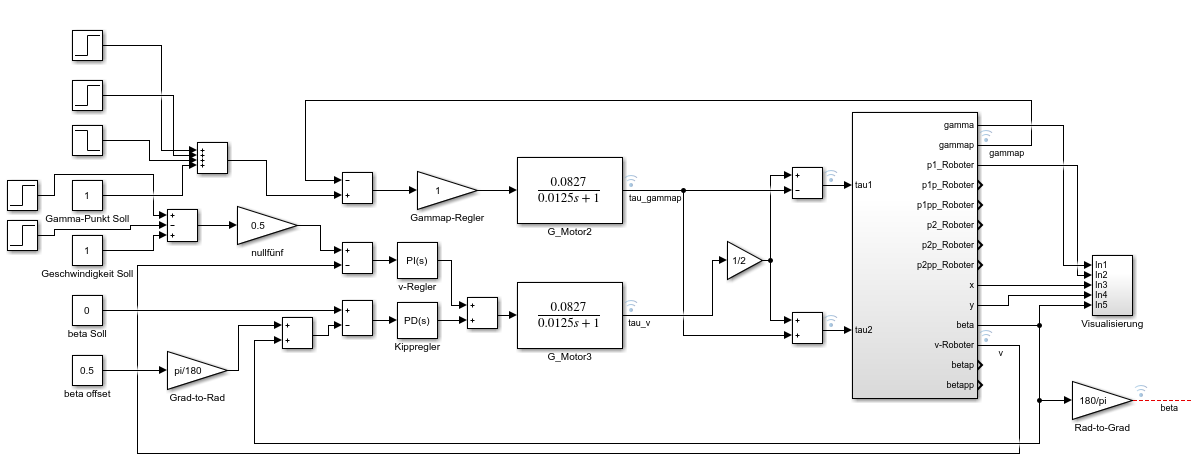
\includegraphics[width=1.0\textwidth]{images/SimulinkReglerstruktur.png}
	% caption ist die Bildunterschrift, taucht auch im Abbildungsverzeichnis auf
	\caption{Simulinkmodell \newline(Quelle: Eigenes Modell)}
	\label{bild_1.1} % über das label kann man aus dem Text auf das Bild verweisen
\end{figure}

\subsubsection{Kippregler}
Das System ist instabil, der Roboter würde einfach umfallen. Um dies zu verhindern wird ein Kippregler ausgelegt.

Das Wurzelortskurvenverfahren zum Entwerfen des Kippreglers bietet sich an, da das gegebene System an das Zeitverhalten des geschlossenen Kreises sowie der Lage des dominierenden Polpaares gebunden ist.  Dabei wird die Übertragungsfunktion des offenen Kreises $G_{Strecke}(s)\cdot G_{Regler}(s)$ gebildet und die entsprechende Wurzelortskurve betrachtet. Aus dem qualitativen Verlauf der Wurzelortskurve ist bekannt, wie sich die Pole, in Abhängigkeit der Reglerverstärkung k, verändern. Sie liegen für k=0 im Ursprung ihres Astes und bewegen sich für steigende Verstärkungen an ihm entlang, bis sich der Pol für k→ ∞ im Unendlichen befindet oder durch eine in der Nähe befindliche Nullstelle kompensiert wird. Letztendlich müssen dem Regler eine oder mehrere Nullstellen gegeben werden, welche die Äste der Wurzelortskurven des offenen Kreises verändern. Dadurch soll das dominierende Polpaar durch eine bewusste Wahl der Reglerverstärkung k in den gewünschten Bereich der komplexen Ebene gelangen und damit das System stabilisieren. Im Optimalfall werden dadurch die restlichen Polstellen so weit nach links verschoben, dass sie einen möglichst geringen Einfluss auf das System haben und das dominierende Polpaar alleine das Verhalten bestimmt.

Die Berechnung ergab einen Pol der Dynamik bei $-14,05$. Um diesen zu Eliminieren wurde ein PD - Regler verwendet.

Die Koeffizienten lauten:
\begin{itemize}
	\item $ T_{V}=0,07$
	\item $ k_{PD}=-60$
\end{itemize}
\subsubsection{Geschwindigkeitsregler}
Da der Kippregler keinen Offset des Winkels regeln kann wird auch zum Stehen ein Geschwindigkeitsregler benötigt. Des weiteren wird durch ihn auch die Geradeausfahrt ermöglicht. Der Sollwert der Geschwindigkeit soll schnell und möglichst genau erreicht werden.
Verwendet wurde ein PI - Regler. Ausgelegt wurde hier mittels der Einstellregeln von Ziegler-Nichols nach dem Stabilitätsrand.
\begin{itemize}
	\item $ T_{N}=0,4$
	\item $ k_{PI}=4,50$
\end{itemize}
Die Simulation wies starkes Schwingen auf, daraufhin wurde der Anteil des Integrators gesenkt, bzw. $ T_{N}=2,66$ erhöht.
\subsubsection{Rotationsgeschwindigkeitsregler}
Um auch das Fahren von Kurven zu ermöglichen, wird ein Rotationsgeschwindigkeitsregler, ein einfacher P-Regler verwendet. Die Verstärkung $k_{P}=1$ muss in einem Experiment getestet werden und kann gegebenenfalls erhöht werden.
\subsubsection{Positionsregler}
Der Roboter soll vorgegeben Koordinaten anfahren können und  diese auch halten. Dafür sorgt der Positionsregler. Ausgeführt wurden 3 Modi:
\begin{itemize}
	\item Vorwärtsfahrt
	\item Vorwärts-/Rückwärtsfahrt
	\item Vektorregelung
\end{itemize}

Der Zielvektor in Bezug auf den Roboter wird über Koordinatentransformation ermittelt. Mit dem atan2(y,x) wird dann die Winkeldifferenz berechnet. Die translatorische Geschwindigkeit wird über den Abstand skaliert und mit max $|0,5| \dfrac{m}{s}$ beschränkt. Die Winkelgeschwindigkeit ist auf $\pm6 \dfrac{rad}{s}$ beschränkt.
\begin{itemize}
	\item $k_{PGamma} = 4$
	\item $k_{PDistanz} = 0,5$
\end{itemize}
Die Verstärkungen wurden so gewählt, das der Roboter Ziele in $1m$ Entfernung gut erreicht. Zu weiter entfernten Zielen fährt er sehr direkt.
\subsubsubsection{Vorwärtsfahrt}
Der Roboter fährt nur Vorwärts und dreht sich in die Richtung in welcher der Winkel kleiner ist.
\subsubsubsection{Vorwärts-/Rückwärtsfahrt}
Der Roboter fährt bei einem Winkel von unter $\pm90^{\circ}$ vorwärts bei einem Winkel darüber rückwärts zum Ziel.
\subsubsubsection{Vektorregelung}
Der Roboter dreht sich wie bei der Vorwärtsfahrt. Die translatorische Geschwindigkeit wird über das Skalarprodukt zwischen Zielvektor und Robotervektor $[1;0]$ berechnet. Steht der Roboter also zu Beginn rückwärts zum Ziel, fährt der Roboter zunächst auch rückwärts bis er sich auf $\pm90^{\circ}$ gedreht hat.


\newpage
